% !TeX root = ../my-thesis.tex
\chapter{Verwendete Geräte und Tools}
\section{Vorstellung der Test-App für diese Arbeit}
Im Rahmen dieser Arbeit, wurde die \glqq EnergyEfficience\grqq{} App entwickelt. In dieser App wurden verschiedene Implementationen von Algorithmen umgesetzt, mit deren Hilfe Laufzeit- und Energieeffizienz dieser Berechnungen gemessen werden kann.
Die \glqq EnergyEfficience\grqq{} App wurde auf Basis der Android \ac{sdk} 30 entwickelt, welche die zum Zeitpunkt der Erstellung dieser Arbeit die aktuellste Android API ist und somit für Android 11 lauffähig ist. Für die Programmierung selbst wurde ausschließlich mit Java gearbeitet. Allerdings ist Kotlin jetzt schon offiziell die empfohlene Programmiersprache für die Androidentwicklung, da die Bereitstellung der neuen \ac{sdk}'s und Android Support Bibliotheken immer stärker auf das Motto \glqq Kotlin-first\grqq{} \cite{kotlin-first} umgestellt wird. Inwiefern die Java Unterstützung für zukünftige \ac{sdk} Versionen bestehen bleibt, ist zum aktuellen Zeitpunkt nicht absehbar.
Für die persistente Speicherung von beispielsweise Testdaten und Nutzereinstellungen wurde die Room Persistence Library in der Version 2.2.5 genutzt.
\begin{figure}[H]
	\begin{center}	 
	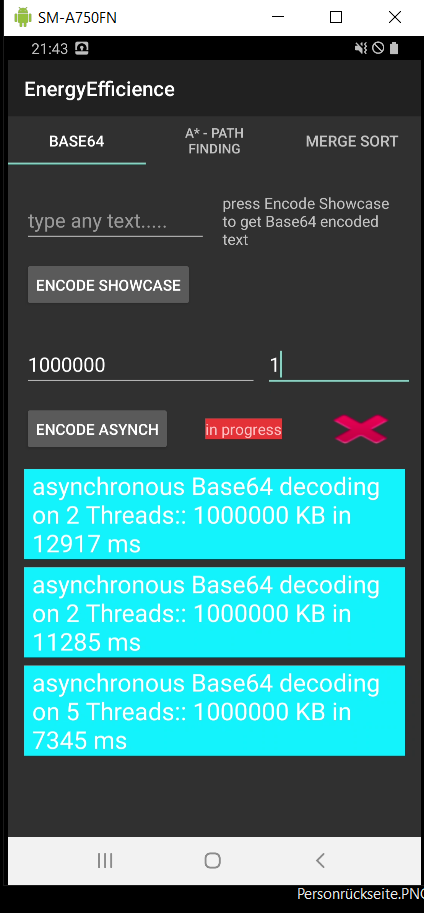
\includegraphics[scale=0.5]{base64Pic}
	\caption{MainActivity der EnergyEfficience App (eigene Abbildung)}
	\label{fig:MainActivity} 
	\end{center}
\end{figure}
In \autoref{fig:MainActivity} ist das \ac{ui} der Launch Activity der App zu sehen. Über ein dreiteiliges Tab Layout Menü sind drei verschiedene Fragmente erreichbar, welche jeweils einen Algorithmus thematisieren. Die Fragmente sind über einen View Pager und einen Fragment State Adapter mit dem Tab Layout gekoppelt. Das Base64 Fragment implementiert einen einfachen Base64 Encoder. Über die Schaltfläche \glqq ENCODE SHOWCASE\grqq{} wird der Text aus dem darüber gelegenen Eingabefeld in das entsprechende Base64-Format kodiert und in der rechts angrenzenden TextView ausgegeben. Die für die Messung relevanten Berechnungen lassen sich über den \glqq ENCODE ASYNCH\grqq{} Button starten. Bevor dies geschieht, sollte in das links darüber gelegene Textfeld die Größe des zu kodierenden Strings angeben werden. Dabei ist ist die Einheit \ac{kb} und es sollte darauf geachtet werden, dass aus implementationstechnischen Gründen die Mindestgröße von 10000 \ac{kb} nicht unterschritten wird. 
Über das rechts daneben platzierte Textfeld lässt sich die Anzahl der Threads festlegen, welche zur parallelen Ausführung der Kodierung genutzt werden soll. Die detaillierte Implementierung dieser Parallelität wird in Kapitel 4.3 \glqq Thread Pool Implementierung zur effizienten Ressourcenverwaltung\grqq{} beschrieben.\todo{Verweis auf Kapitel} Während der Laufzeit der Kodierung erscheint eine rot unterlegte \glqq in progress\grqq{} Meldung, welche nach Terminierung wieder verschwindet. Die Laufzeitdaten und Parameter des Durchlaufs werden anschließend in blau gestalteten Textboxen innerhalb einer scrollbaren Recycler View dargestellt. Mithilfe des roten Kreuzes kann die Recycler View wieder geleert werden.
\begin{figure}[H]
\begin{center}
	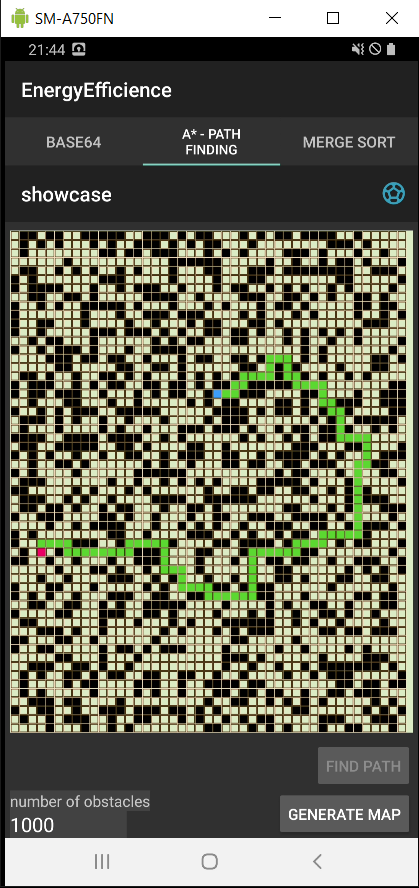
\includegraphics[scale=0.5]{ASternPic}
	\caption{A*-Path finding Fragment (eigene Abbildung)}
	\label{fig:Pathfinding} 
\end{center}
\end{figure}
Im A*-Path finding Fragment wurde eine Implementierung des A* Pathfinding Algorithmus umgesetzt. Die \ac{ui} ist in \autoref{fig:Pathfinding} zu sehen. Über die Schaltfläche \glqq GENERATE MAP\grqq{} wird eine zweidimensionale Rasterkarte mit zufällig generierten Start- und Endpunkten einer Route und beliebig vielen Hindernissen erstellt. Nach Betätigung der \glqq FIND PATH\grqq{} Schaltfläche wird, falls vorhanden, der kürzeste Weg zwischen Start- und Endpunkt ermittelt und anhand einer grünen Markierung gekennzeichnet.

In \autoref{fig:MergeSort} ist auf der einen Seite das Merge Sort Fragment zu sehen, welches zur Veranschaulichung der verschiedenen Merge Sort Varianten dient und auf der anderen Seite die Merge Sort Activty, welche für die Messung notwendige Anpassungen enthält. 
\begin{figure}[H]
\begin{center}
	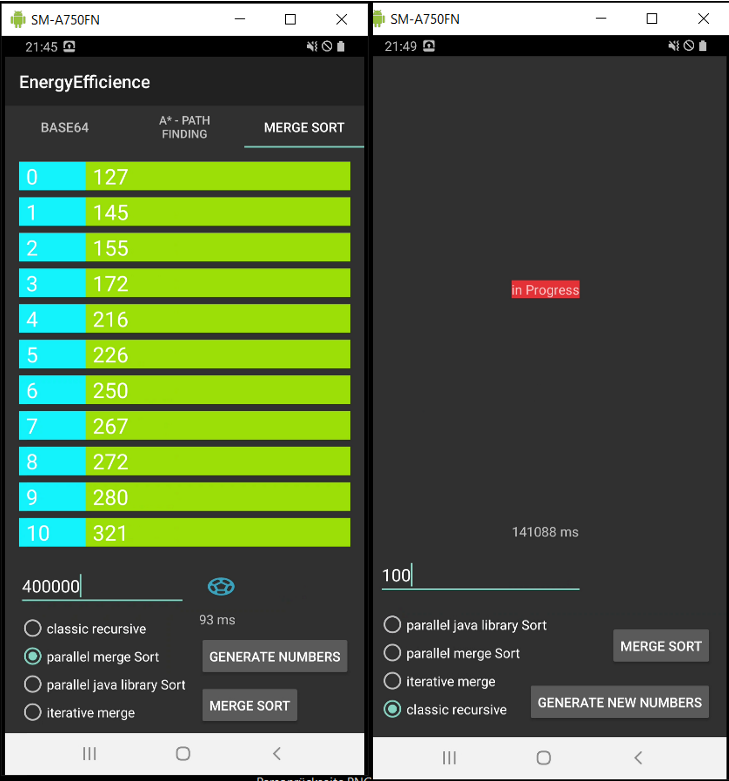
\includegraphics[scale=0.5]{MergeSort}
	\caption{MergeSort Fragment und Activity zur Messung (eigene Abbildung)}
	\label{fig:MergeSort} 
\end{center}
\end{figure}
Über das Textfeld kann eine beliebige Anzahl von Nummern festgelegt werden, welche durch den Algorithmus sortiert werden soll. Es wird empfohlen, dabei die Obergrenze von 5 \ac{mio} nicht zu überschreiten, da es bei der Allokation von Arbeitsspeicher für Datenstrukturen wie Arrays oder Listen mit so vielen Elementen zu Out of Memory Erros kommen kann. Diese führen unweigerlich zum Absturz der Applikation. Durch betätigen der \glqq GENERATE NUMBERS\grqq{} Schaltfläche werden dieser Anzahl entsprechend viele Zufallszahlen zwischen 0 und 9000000 in zufälliger Reihenfolge generiert und Recycler View dargestellt. Dabei gibt der blau hinterlegte Index die Position der Zahl im internen Array an. Über die 4 Radio Buttons kann zwischen verschiedenen Sortierverfahren gewählt werden. Für die Untersuchung im Rahmen dieser Arbeit sind der klassische, rekursive Merge Sort, der iterative Merge Sort und der parallele Merge Sort relevant. Über die \glqq MERGE SORT\grqq{} Schaltfläche kann die Sortierung gestartet werden. Auch hier wird nach Terminierung der Berechnung die Laufzeit in \ac{ms} ausgegeben. Die Elemente in der Recycle View werden anschließend der neuen Sortierung entsprechend aktualisiert. Die Einschränkung durch den vergleichsweise geringen Arbeitsspeicher auf mobilien Geräten verhindert die Generierung von ausreichend vielen Testdaten um eine für Messungen günstige Laufzeit zu erreichen. Daher wurde eine weitere Activity erstellt, um dieses Problem für längere Messungen zu umgehen. Auf der rechten Seite von \autoref{fig:MergeSort} ist zu erkennen, dass das \ac{ui} bis auf das Fehlen der Recycler View einen ähnlichen Aufbau wie das Merge Sort Fragment hat. Hierbei ist jedoch zu Beachten, dass über das Textfeld nicht die Anzahl der Elemente eingestellt wird, sondern die Anzahl der Iterationen einer Sortierung. In jeder Iteration werden 3 \ac{mio} Zahlen sortiert. Dieses Vorgehen verhindert die gleichzeitige Allokation von zu viel Heap Speicher und somit Out of Memory Errors und gewährleistet außerdem eine beliebig andauernde Laufzeit für die Messung. Des weiteren bleiben die Testdaten im Gegensatz zum Merge Sort Fragment konstant, da 3 \ac{mio} Zahlen mithilfe einer Room Database persistent gespeichert werden. Über die Schaltfläche \glqq GENERATE NEW NUMBERS\grqq{} werden 3 \ac{mio} neue Zufallszahlen zwischen 0 und 9 \ac{mio} generiert und in die Datenbank gespeichert werden. Über das blaue, kreisförmige Icon des Merge Sort Fragments, ist diese Activty zu erreichen. Nach Betätigung dieses Icons, kann es einige Sekunden dauern, bis die Actvity einsatzbereit ist, da das Laden von 3 \ac{mio} Elementen aus der Datenbank sehr zeitkritisch ist.
\section{Gerätespezifikationen und Battery Historian zur Messdatenermittlung}

Als Testgerät wurde das Samsung Galaxy A7 aus dem Jahr 2018 gewählt. Es besitzt 64 ac{gb} Festplattenspeicher und 4 ac{gb} Arbeitsspeicher. Der Akku besitzt eine Kapazität von 3300 \ac{mAh}. Bei dem 6 Zoll großen Display handelt es ich um einen Super-AMOLED mit einer Auflösung von 1080 x 2220 Pixel bei einer Pixeldichte von 411 \ac{ppi} \cite{smartphone-data}. Die \ac{cpu} ist ein Achtkernsystem mit der Architektur eines Exynos 7885 \ac{soc} von Samsung.  Diese Architektur besteht zum einen aus 2 schnellen Cortex-A73 Rechenkernen mit 2,20 \ac{ghz} und zum anderen aus 6 stromsparenden Cortex-A53 Kernen mit jeweils 1,6 \ac{ghz} Taktfrequenz. Exynos ist eine \ac{soc} Familie, deren Mikroprozessorkomponenten auf der ARM-Architektur basieren. Diese Architektur zeichnet sich durch einen effizienten Befehlssatz aus, welche eine kompakte Implementierung in einem \ac{ascii} - Design erlaubt und daher für Optimierungen im Bereich der Stromaufnahme sehr gut geeignet ist. Dieses Design wurde ursprünglich vom britischen Unternehmen ARM entwickelt. Große Unternehmen wie Apple, Huawei, Qualcomm oder Samsung besitzen Lizenzen für diese Architektur und können daher Hauseigene Lösungen mit dieser Technik für ihre Geräte entwickeln \cite{cpu-data}. Die mit dieser Architektur einhergehenden Besonderheit, dass Kerne aus 2 verschiedenen Leistungsklassen verbaut werden, spiegelt sich auch in den Messergebnissen der Untersuchung in Kapitel 3 \glqq Energieeffizientes Multithreading\grqq{} wieder. \todo{Kapitelverweis einbauen}

Zur Messung des Strom- und Spannungsverlaufs des Akkus während der Ausführung der Berechnungen wurde das Programm Battery Historian in der Version 3.0 genutzt. Um dieses Tool nutzen zu können, ist eine aktuelle Docker Umgebung nötig. 

Im Rahmen dieser Arbeit wurde die Version v19.03.12 genutzt. Bei Docker handelt es sich um eine Anwendung zur Erstellung und Verwaltung von sogenannten Linux Containern. Dies ermöglicht eine einfache und schnelle Installation und Skalierung von Software jeglicher Art. Sofern eine Installation der Docker Engine vorhanden ist, lassen sich so neue Softwareinstanzen eines beliebigen Programms unabhängig vom installierten Betriebssystem und vorhanden Bibliotheken mit wenig Installationsaufwand aufsetzen. Alle für die Installation nötigen Konfigurationen werden hierbei durch ein Docker Image vorgegeben und müssen nicht mehr manuell umgesetzt werden. Virtuelle Maschinen liefern zwar einen Ähnlichen Komfort, sind jedoch vergleichsweise ressourcenaufwendig, da Hier ganze Betriebssysteme mit hohem Speicherbedarf installiert werden. Die Docker Engine hingegen ermöglicht einen direkte Zugriff auf den Kernel des Host-Betriebssystems und spart somit Speicher und ist wesentlich schneller in der Ausführung als eine herkömmliche virtuelle Maschine \cite{Docker}.  In Verbindung mit zusätzlichen Tools wie Kubernetes, kann die Skalierung und Verwaltung der Docker Container und somit auch der eigenen Softwareinstanzen fast vollständig automatisiert werden \cite{Kubernetes}.

Soblad das aktuelle Docker Image von Battery Historian läuft, ist es möglich, die von Android gesammelten Logdateien bezüglich des Batteriestatus in einer \ac{html} Visualisierung darzustellen. Informationen über den Energieverbrauch und Statistiken über die Nutzung von sämtlichen Hardwarekomponenten des Gerätes werden permanent im Hintergrund gesammelt. Hierzu wird unter anderem das Tool Batterystats genutz, welches in das Android Framework integriert ist \cite{batteryhistorianandroid}. Mithilfe der \ac{adb} \footnote{die \ac{adb} ist ein Schnittstellen Programm zwischen Computer und Androidgerät zur Ausführung von Befehlen und zur Übertragung von Dateien} ist es möglich, diese Logdaten in ein ZIP-Dateiformat zu komprimieren und auf ein anderes Gerät zu laden. Hierfür wird der Befehl \emph{adb bugreport bugreport.zip} genutzt \cite{batteryhistorian}. 

In Abbildung \ref{fig:Voltage} ist die grafische Darstellung dieser Logdateien zu sehen. Die horizontal verlaufenden farbigen Balken kennzeichnen die Aktivität verschiedener Komponenten des Smartphones, welche zum jeweiligen Zeitpunkt Strom verbrauchen. So lassen sich \ac{cpu} Aktivitäten, Wakelocks oder \ac{wifi} Aktivitäten nachvollziehen. Für Netzwerkspezfische Datensätzte wie \glqq Mobile signal strength\grqq{} oder \glqq Wifi signal strength\grqq{} nimmt der Balken in Abhängigkeit der Signalstärke verschiedene Farben an. So steht ein Grün für optimale Signalstärke und rot für eine schlechte Verbindung. Sehr nützlich für die Untersuchung sind vor allem die Informationen zur aktuellen Betriebstemperatur des Chips und die Anzeige von Benutzerimplizierten Wakelocks. Die Betriebstemperatur ist ein signifikanter Faktor, der die Leistungsfähigkeit der \ac{cpu} beeinflusst und daher während der Messungen möglichst konstant gehalten werden muss, um vergleichbare Ergebnisse zu erhalten. Um die Lebensspanne der Chips zu erhöhen, wird bei zu hoher Betriebstemperatur die Frequenz der Rechenkerne herabgesetzt um die Hardware zu schonen.

Über ein Dropdown-Menü rechts oberhalb des Diagramms, lassen sich verschiedene Graphen Anzeigen. In \autoref{fig:Voltage} ist der Voltage Graph zu sehen, welcher den Spannungsverlauf in \ac{mV} über die Ziet darstellt. Das Tool zeichnet Messwerte im Intervall von 30 Sekunden auf. Daher sind relativ lang andauernde Messungen über mehrere Minuten notwendig, um verwertbare Wertereihen zu erhalten. Die Spannung wird für jedes 30 Sekundenintervall als Spannungsbereich mit Ober- und Untergrenze angegeben. In \autoref{fig:Voltage} ist beispielsweise ein Messpunk ausgewählt mit einer Spannung, die im aktuellen 30 Sekundenintervall zwischen 4127 \ac{mV} und 3986 \ac{mV} liegt. Für die Berechnungen für die Untersuchung dieser Arbeit wurden stets die Mittelwerte dieser Spannungsbereiche ermittelt und genutzt. Um Werte für die Stromstärke in Abhängigkeit von der Zeit einsehen zu können, muss entweder der Graph Battery Level oder Coulomb charge genutzt werden. Auch hier werden die Werte in Intervallen von 30 Sekunden angezeigt. Allerdings wird hier ein genauer Wert in \ac{mA} angegeben, welcher neben dem Wert für den aktuellen Füllstand des Akkus in \ac{mAh} als \glqq Charge rate\grqq{} abzulesen ist. Mithilfe der beiden Graphen für den Spannungs- und Entladestromverlauf kann die elektrische Leistung über die Zeit abgebildet werden. Anschließend kann durch Integration dieses Graphen der Energieverbrauch insgesamt als verrichtete elektrische Arbeit ermittelt werden. Dieses Vorgehen wird in den folgenden Kapiteln mit der Anwendung auf die Messwerte näher beschrieben. Alle Messungen wurden unter möglichst identischen Grundvoraussetzungen durchgeführt. Es wurde stets das gleiche Gerät verwendet. Jede Messung wurde mit identischen Akkufüllstand gestartet. Außerdem wurde darauf geachtet, dass während den Messungen keine Netzwerkverbindungen aktiv waren. Einstellungen wie Bildschirmhelligkeit oder Betriebsmodus wurden nicht variiert. Im Zeitraum der Untersuchung wurden außerdem keine Updates des Betriebssystems zugelassen um eine möglichst konstante Laufzeitumgebung zu gewährleisten.

\begin{figure}
\begin{center}
	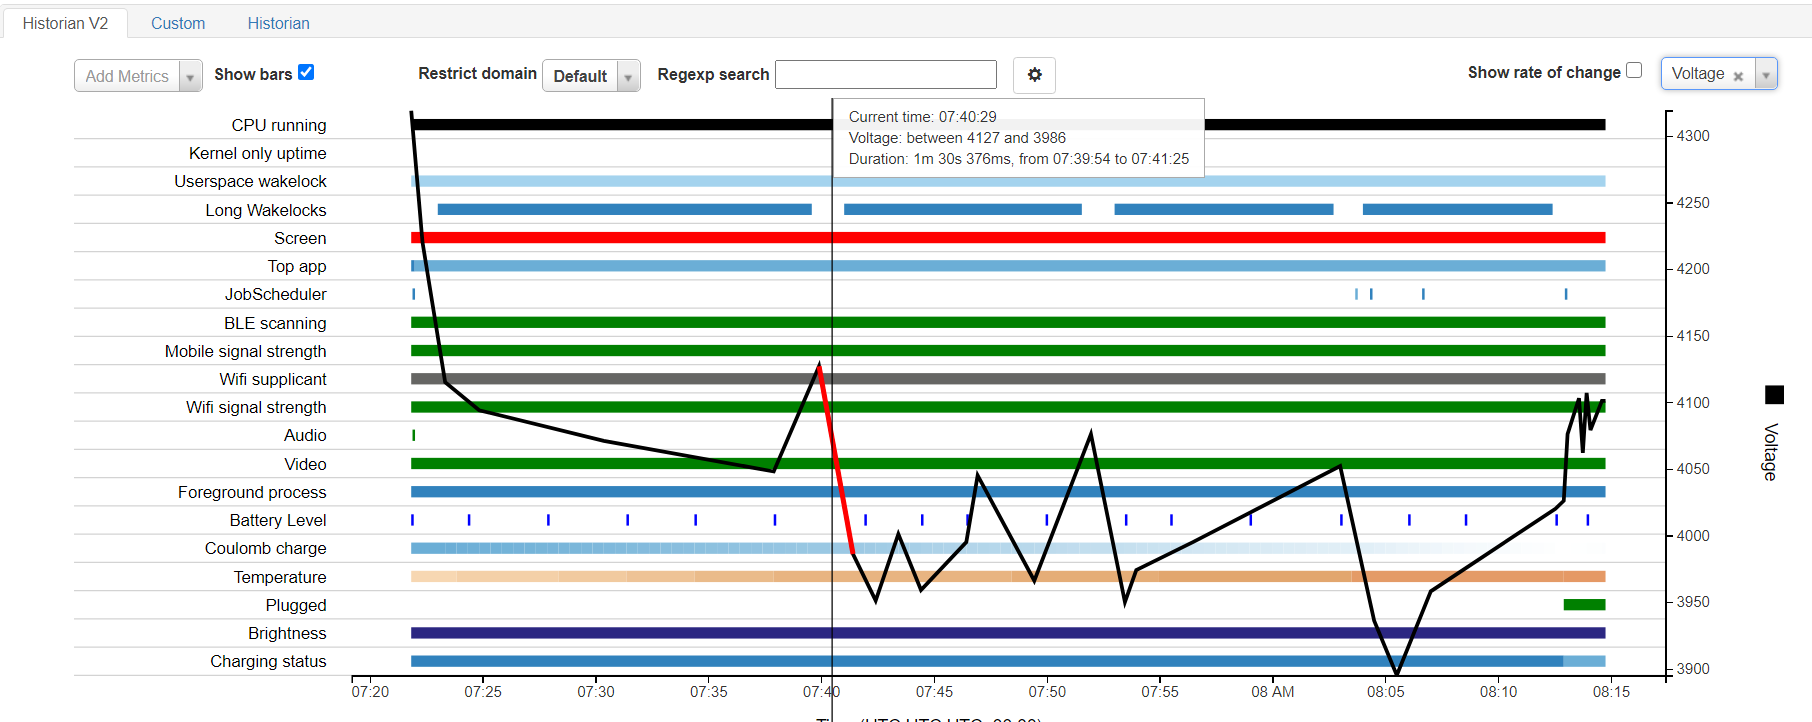
\includegraphics[scale=0.3]{Voltage}
	\caption{Battery Historian Benutzeroberfläche mit Spannungsverlauf \glqq Voltage\grqq{} (eigene Abbildung)}
	\label{fig:Voltage} 
\end{center}
\end{figure}
